\documentclass[10pt,a4paper]{article}
\usepackage[utf8]{inputenc}
\usepackage{amsmath}
\usepackage{amsfonts}
\usepackage{amssymb}
\usepackage{tikz}
\usepackage{hyperref}

\begin{document}
\paragraph{Conseil au lecteur}
	Si vous n'êtes pas familier avec les flexagones, les 
	\href{https://www.youtube.com/playlist?list=PLNefH6S6myiO_5HBDdtP_r_LlCcVwA04I}{vidéos} 
	 de Mickaël Launay sont d'une qualité que je ne pourrait égaler dans un compte-rendu écrit.
	
	\section{Représentation}
		En numérotant chaque face du flexagone, il est assez naturel de construire le graphe de relation suivant:
		
		\begin{list}{•}{}
		\item Les sommets représentent les faces par leur numéro
		\item Deux sommets A et B sont liés ssi les faces qu'il représentent sont voisines dans le flexagone, i.e.
			il est possible de voir les faces A et B de part et d'autre du flexagone simultanément
		\end{list}
		
		Exemple pour les flexagones à 3, 4, 5 faces:
	\begin{center}
		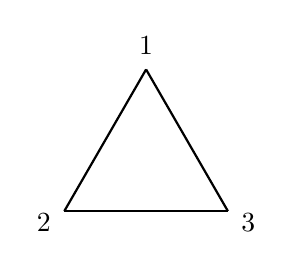
\begin{tikzpicture}[thick,scale=0.3]
		    \foreach \x in {1,2,...,3} {
		        \draw (120*\x - 30 :4) -- (90+120*\x:4);
		        \draw (-30+120*\x:5) node{\x}-- (-30+120*\x:5);
				};
		\end{tikzpicture}
		\\
		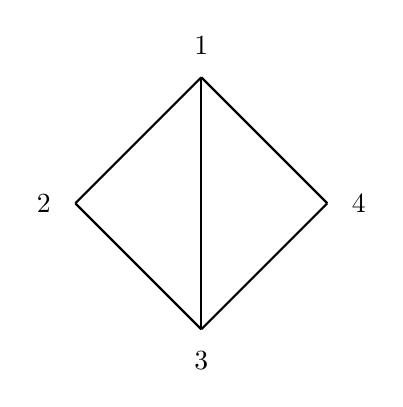
\begin{tikzpicture}[thick,scale=0.4]
		    \foreach \x in {1,2,...,4} {
		        \draw (90*\x:4) -- (90+90*\x:4);
		        \draw (90*\x:5) node{\x}-- (90*\x:5);
				};
				\draw (90:4) -- (270:4);
		\end{tikzpicture}
		\\
		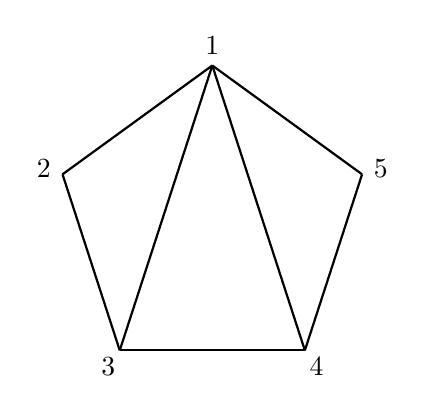
\begin{tikzpicture}[thick,scale=0.5]
		    \foreach \x in {1,2,...,5} {
		        \draw (18+72*\x:4) -- (18+72+72*\x:4);
		        \draw (18+72*\x:4.5) node{\x}-- (18+72*\x:4.5);
				};
				\draw (90:4) -- (306:4);		
				\draw (90:4) -- (234:4);
		\end{tikzpicture}
	\end{center}
\newpage
	\paragraph{}
		On observe de manière générale que ces graphes sont des triangulations de polygones, ici représentés réguliers. En effet, l'opération qui consiste à ajouter une face au flexagone se représente de façon très agréable:\\
		Il suffit d'accoler un triangle supplémentaire à la triangulation.
	
		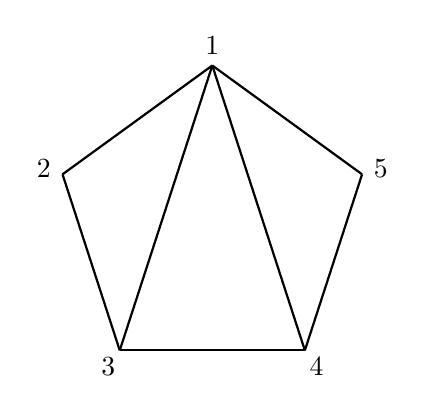
\begin{tikzpicture}[thick,scale=0.5]
		    \foreach \x in {1,2,...,5} {
		        \draw (18+72*\x:4) -- (18+72+72*\x:4);
		        \draw (18+72*\x:4.5) node{\x}-- (18+72*\x:4.5);
				};
				\draw (90:4) -- (306:4);		
				\draw (90:4) -- (234:4);
		\end{tikzpicture}

\end{document}